% 
\documentclass[a4paper]{article}
\usepackage[OT1]{fontenc}
\usepackage{hyperref}
\usepackage{Sweave}
\usepackage{graphicx}
\graphicspath{{figures/}}
%\usepackage{float}
\usepackage{wrapfig}
%\usepackage{subfigure}
%% Package to linebreak URLs in a sane manner.
\usepackage{url}
%% Define a new 'smallurl' style for the package that will use a smaller font.
\makeatletter
\def\url@smallurlstyle{%
  \@ifundefined{selectfont}{\def\UrlFont{\sf}}{\def\UrlFont{\small\ttfamily}}}
\makeatother
%% Now actually use the newly defined style.
\urlstyle{smallurl}
%% Define 'tinyurl' style for even smaller URLs (such as in tables)
\makeatletter
\def\url@tinyurlstyle{%
  \@ifundefined{selectfont}{\def\UrlFont{\sf}}{\def\UrlFont{\scriptsize\ttfamily}}}
\makeatother
%% Make margins less ridiculous
\usepackage{fullpage}
%% Make URLs clickable
%\usepackage[colorlinks, bookmarks=false]{hyperref}
%\usepackage[colorlinks, bookmarks=true]{hyperref}
%% Since I'm using the LaTeX Makefile that uses dvips, I need this
%% package to make URLs break nicely
\usepackage{breakurl}
\usepackage{todonotes}
\usepackage{amsmath,amsfonts}
\numberwithin{equation}{subsection}
%%\usepackage{nonfloat}
\usepackage{bbm}
\usepackage{setspace}
\onehalfspacing
\usepackage{tabularx}
\begin{document}

\title{Mining of Android SCM}
\author{Pavel Senin}

\maketitle

\begin{abstract}
Both, software product improvement and software process improvement, require in-depth understanding 
of current project state. Here I present an approach for exploration of a software repository by 
using Software Trajectory code. I will explore Android SCM system\ldots

\end{abstract}

\section{Introduction}
According to the Android home website, \url{http://source.android.com/}: ``Android is an 
open-source software stack for mobile phones and other devices''.

Initial developer of the software, Android Inc. was purchased by Google in in 2005. In November 2007 
the Open Handset Alliance, a consortium of 84 companies, announced availability of the 
Android Software Development Kit (SDK). The open Open Handset Alliance is formed of hardware, 
software, and telecommunication companies and devoted to advancing of open standards for mobile 
devices. The Android code is open-source and released under the Apache License; it is a complete 
mobile platform built on the monolithic Linux 2.6 kernel. 

\begin{wrapfigure}{l}{0.5\textwidth}
   \begin{center}
   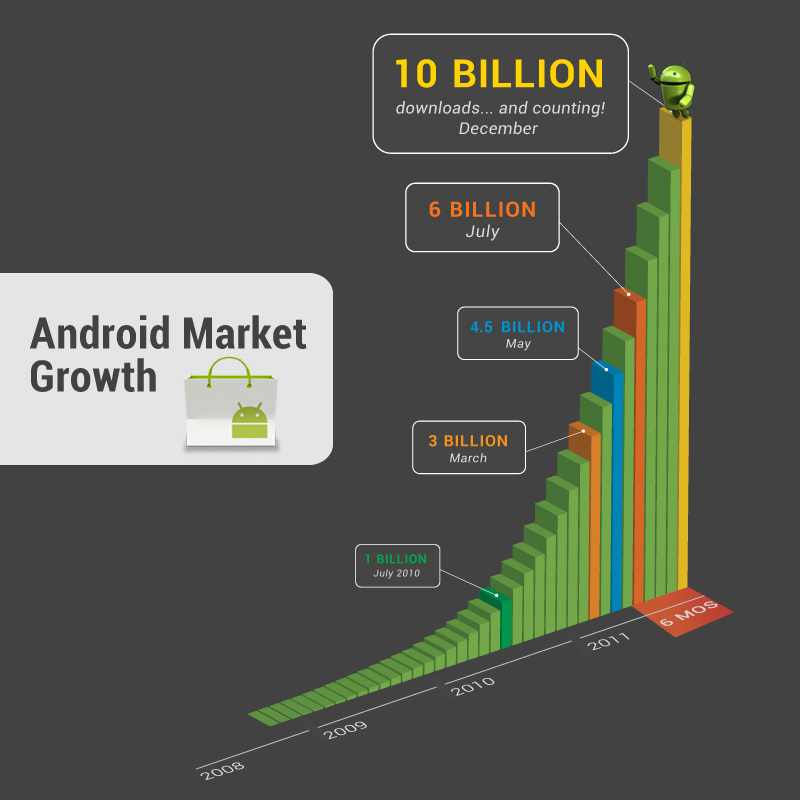
\includegraphics[scale=0.3,bb=0 0 800 800,width=0.48\textwidth]{graph_only_3}
   \end{center}
   \caption{The Android store downloads timeline.}
   \label{fig:android_downloads}
\end{wrapfigure}


The Android platform provides a set of development tools, debugger and a true emulator.
There are the Eclipse plugin, a set of libraries, a multimedia user interface, and a core set of 
phone applications. The Android application model alleviates the cost of software development 
by allowing extending, replacing, and reusing of existing software components. The Dalvik virtual 
machine, which is the part of Android distribution, provides a way to maximize application 
portability, performance and security.

Currently, the Android Open Source Project (AOSP) is led by Google and includes not only the 
original members of OHA but many other companies. The role of AOSP is to maintain and develop 
Android.

Including Beta, there were 10 major releases of Android as well as a number of intermediate 
releases. In December 2011 there were registered 10 billions of downloads from Android store. 

\section{Contributors}
Currently, Android code is hosted at Goggle Git. There are 1771667 changes 
registered in the repository. First change commit to Android repository dates back 
to Monday January 12th 1970, 14:46:40 and belongs to Upstream, while the last change
within the analyzed data set belongs to to Guy Zadickario and dated 
Tuesday June 21st 2011, 12:41:41.


\section{Source code}
As per January, 1, 2012 Android repository contains a total of 26851267 lines of source code in 
152225 files. 

\begin{table}
  \caption{Android repository snapshot source code metrics.}
  \begin{tabularx}{\textwidth}{ | X | r | r | r | r | r |}
  \hline                       
  Nb. files & Language & Total lines & Source & Blanks & Comments \\
  \hline 
  Assembly &3391 & 565314 & 426104 & 60673 & 98215 \\
  IDL & 78 & 7926 & 7174 & 752 & 640 \\
 Perl & 348 & 105024 & 75877 & 13999 & 18975 \\    
  CSS & 224 & 38417 & 30687 & 5899 & 2033 \\
  XML & 10090 & 5963665 & 5762297 & 59093 & 143243 \\   
  Matlab & 889 & 62911 & 51323 & 10715 & 3911 \\
  Text & 7563 & 1669710 & 0 & 93271 & 1576439 \\
  FlashParameter & 3 & 364 & 265 & 40 & 59 \\
  C & 42151 & 9979284 & 6676807 & 1278259 & 2363003 \\   
  shell & 3930 & 2476537 & 1986936 & 207861 & 288125 \\  
  JavaScript & 5347 & 866236 & 511330 & 131581 & 225745 \\   
  Java & 251129 & 5265723 & 3152054 & 639535 & 1509917 \\
  HTML & 6209 & 1208415 & 1062506 & 100306 & 61760 \\
  make & 3506 & 512065 & 377850 & 62696 & 71518 \\
  Awk & 21 & 2762 & 1778 & 226 & 871 \\
  SQL & 3 & 454 & 454 & 0 & 0 \\
  Pascal & 160 & 15681 & 2555 & 372 & 13334 \\      
  Python & 912 & 190278 & 132202 & 30889 & 27888 \\ 
  PHP & 180 & 50137 & 39060 & 2268 & 9218 \\
  C++ & 31390 & 9228878 & 6262708 & 1318921 & 1835150 \\   
  Jess & 2 & 246 & 192 & 54 & 0 \\
  CSharp & 66 & 6513 & 5282 & 643 & 596 \\      
  Lisp & 10633 & 493777 & 285826 & 86471 & 176378 \\
  \hline     
  TOTAL & 152225 & 38710317 & 4104524 & 8427018 & 26851267 \\    
  \hline  
  \end{tabularx}
\end{table}


\end{document}
